\documentclass{article}

\usepackage{spconf}
\usepackage{siunitx}
\usepackage{graphicx}
\usepackage{tabularx}
\usepackage{verbatim}
\usepackage[hidelinks]{hyperref}
\usepackage{biograph}
\usepackage{wrapfig}

\title{Raspberry Pi Driven Vision for Autonomous Mobility}
\name{Andrei Tumbar}
\address{Computer Engineering\\
Rochester Institute of Technology\\
at1777@rit.edu}

\begin{document}
\maketitle

\begin{abstract}
Classical computer vision has always been a challenge to implement on embedded systems because of the requirement of fast computational power and system memory. This paper presents a possible solution to realtime computer vision aboard a Raspberry Pi 3B for the purpose of driving an autonomous vehicle.
\end{abstract}

\section{Introduction}

Vision processing is a fairly well developed field that looks at processing images to extract certain features. This can include features such as object edges, object classification, or 3D mesh reconstruction with stereo correlation. One of the major challenges of computer vision in robotics and other embedded systems arises from vast computational requirements.

Many robots that operate from the input of a camera will use some form of computer vision to drive their navigation logic. For example, the Perseverance rover uses a combination of its 6 engineering cameras as well as an inertial measurement unit for path planning and pose estimation \cite{b1}. One of the main challenges with computer vision for robotics and other embedded system arises from the large computational requirements of vision software. While algorithms are parallelizable making graphics processing units (GPUs) highly attractive, power constraints of these robots usually factors into the choice of control.

There has been some work in the past done to implement vision on the Raspberry Pi. \cite{b3} discusses a Raspberry Pi configuration that uses the Raspberry Pi camera module. OpenCV is used to support much of the vision functionality. This project will use a similar hardware configuration, however, will differ in operating system and programming language when comparing to \cite{b3}. Instead, a custom compiled, statically linked version of OpenCV is built as well as a leaned down version Debian Linux operating system is used instead of the one noted in \cite{b3}.

This paper introduces a vision and navigation system aboard a Raspberry Pi 3B. The official Raspberry Pi Camera Module V2 is used for its impressive streaming features and hardware noise reduction. The vision system is meant to drive a small battery powered car around a track. The Raspberry Pi's low power requirements of \SI{3.7}{\watt} at maximum load of all four internal cores makes it a good option for this application \cite{b2}. This paper is divided into three main sections. The background will explain the general design of the car and introduce ideas such control systems used in later sections of the paper. The proposed method section will discuss the specific implementation details of the major components of the car. Finally, the results section will discussed what went wrong, what went right, and future work to continue this project.

\section{Background}

\subsection{TI Cup Car Hardware}

The purpose of this project is to drive a TI Cup Car. This car includes two direct current (DC) motors used to drive the rear wheels as well as a servo motor to control the steering arms. All three motors are driven with a pulse-width modulation (PWM) signal. The DC motors have a base frequency of \SI{10}{\kilo\hertz} while the steering servo uses a frequency of \SI{50}{\hertz}. Due to the low current limitations of a software drivable general purpose input/output (GPIO) pins, the DC motors cannot be switched directly from the pin headers. A motor driver must be used to switch an external power source controlled by a low drive GPIO. This motor driver is an H-bridge circuit able to switch the high current requirement of the DC motors from the external battery under the control of a \SI{3.3}{\volt} GPIO PWM signal.

The generation of these PWM signals is done by an MSP432P401R microcontroller. This microcontroller is capable of generating multiple simultaneous hardware driven PWM signals and can be used to drive multiple motors. The microcontroller is used instead of the Raspberry Pi as the Pi is only able to generate two hardware driven PWM signals and therefore not able to control the car.

\begin{comment}
One of the challenges the Raspberry Pi board for use with this vehicle is the hardware limitations presented by the board. The Raspberry Pi only includes two hardware PWM channels. Each channel may be configured to drive one of two selectable GPIO pins exposed on the Raspberry Pi header. This leaves one of three options: drive both the DC motors with a single PWM signal, drive the DC motors with the hardware PWM and the steering servo with software PWM, command a microcontroller to generate PWM signals
and control all three motors on its own.

The first two options noted above both present problems of their own. The first option is not possible to be implemented on the specific motor driver board as the pins that drive the DC motors only work with one set of the PWM pins on the two channels. Implementing the servo signal using a software driven PWM signal is risky as the response time of a non-realtime kernel like [standard] Linux is too long to generate a reliable and stable square wave. The final option is the most favourable as the PWM signal generation aboard a microcontroller is always hardware driven and the power requirements of the microcontroller are extremely minimal. This option however does add some complexity to the system as the requirement for yet another board is introduced as well as well as a communication protocol between the two boards. The MSP432P401R microcontroller from Texas Instruments is used for the purpose of driving the PWM pins to control the motors. This is the same board used in class and already has PWM libraries written for previous labs as well as testing on these libraries for validity.
\end{comment}

\subsection{Camera, Vision \& Navigation}

The software built to control the vehicle is divided in three main stages:

\begin{enumerate}
\item Capture camera frame
\item Detect and threshold track edges
\item Compute path and control car to stay on path
\end{enumerate}

The first stage involves capturing raw images from the camera. The Raspberry Pi Camera Module V2 will capture raw image frames through a fisheye lens.
The next step will perform vision processing to raw image frames. Processing is divided into small stages. The collection of processing stages is known as the vision pipeline. To perform certain processing steps, the open-source OpenCV library is used. OpenCV is split into independent modules which are can be built as separate static libraries. This allows a user to compile OpenCV with only a subset of its features to keep the code sizes relatively low. This project uses the image processing module (imgproc) as well as the 3D camera calibration module (calib3d) to support its pipeline.

The final stage in the vehicle control process will take processed images from the vision pipeline and plan a path for the car. It will classify track edges as splines and attempt to find a path within the edges of the track. This stage will keep the car on course using the Proportional-Integral-Derivative (PID) control paradigm.

PID is a control method that looks at bringing a generic system to a desired state while keeping overshoot oscillation and steady state error at a minimum. The basic idea is that given a set of inputs, a system can determine its current state and provide controls to the system to bring it into a desired state. In the context of the car, the desired state is a center position on the track and PID will control the steering on the car.

\begin{figure}[htb]
	\centering
	\centerline{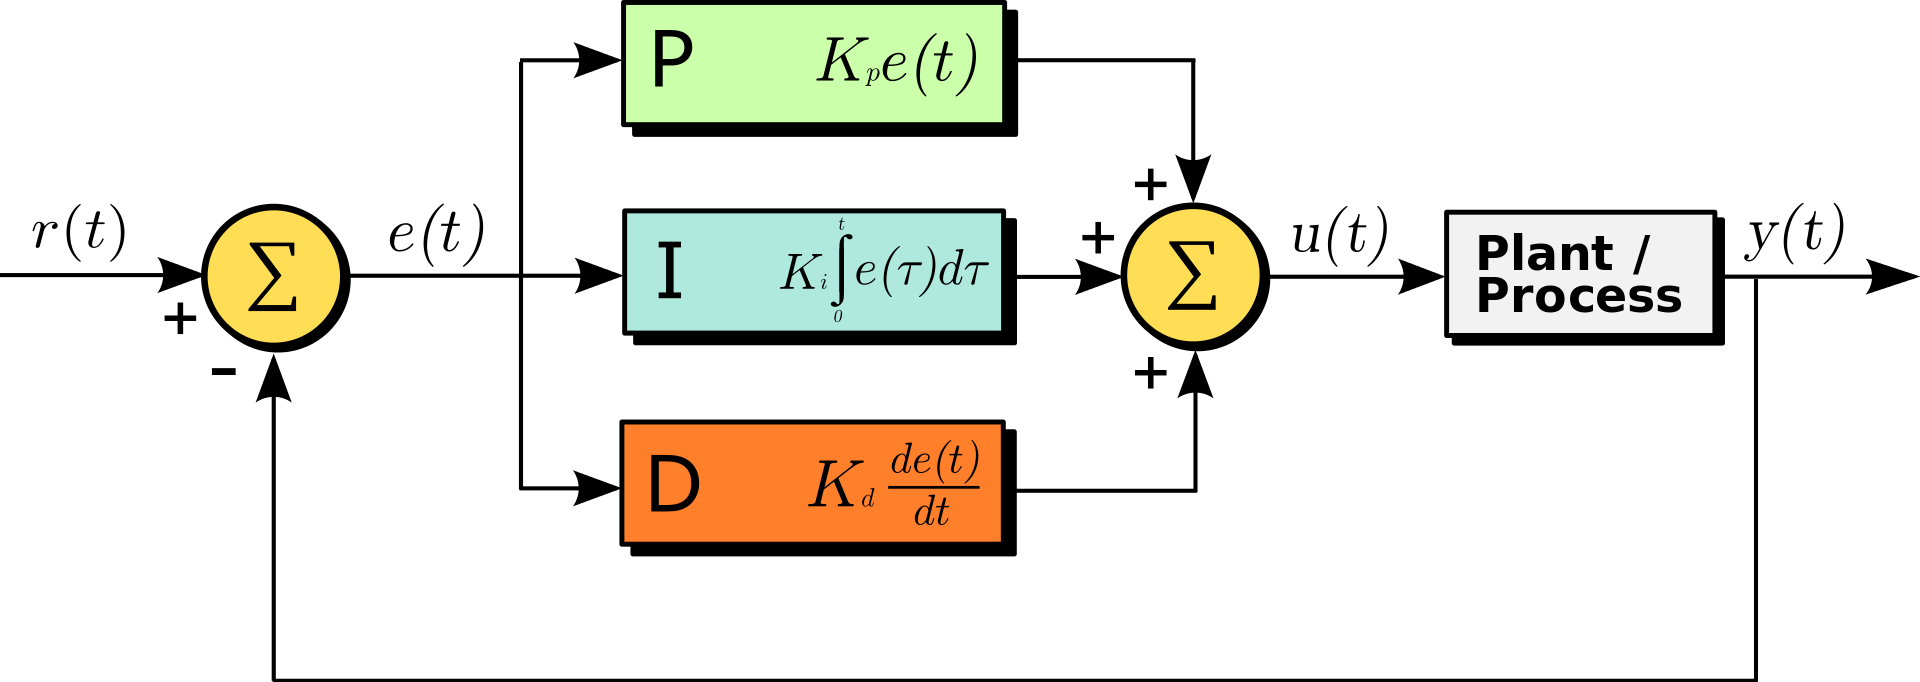
\includegraphics[width=1.0\linewidth]{pid}}
	\caption{Proportional-Integral-Derivative control driving mathematics.}
	\label{fig:pid}
\end{figure}

Fig. \ref{fig:pid} shows the driving mathematics behind the PID control system. $r(t)$ being the current estimated state of the system derived from the various sensors on-board. $e(t)$ is the error, which, as previously mentioned, can be derived from a desired position and a current position. The three terms that control the feed sent back to the robot are weighted by parameterizable coefficients. These coefficient are heavily system dependent and must be manually tuned depending on physical characteristics of the robot and control algorithm. The three parameters, $K_p$, $K_i$, and $K_d$ each react on the error correction of the robot in their own unique way. Here is a table of the effects each coefficient has on the error response of the robot.

\begin{table}[htb]
	\renewcommand{\arraystretch}{1.2}
	\begin{tabularx}{\columnwidth}{|c|>{\raggedright\arraybackslash}X|>{\raggedright\arraybackslash}X|}
		\hline
		Coefficient & Too low & Too High \\
		\hline
		$K_p$ & System will not reach target state before it becomes unstable. & System will oscillate around the target state. \\
		\hline
		$K_i$ & System will undershoot the target during steady state. & System will overshoot the target during steady state. \\
		\hline
		$K_d$ & System will reach the target slowly. & System will attempt to reach the target too quickly and cause overshoot. \\
		\hline
	\end{tabularx}
	\label{tab:pid}
\end{table}

Using the guidelines outlined in table above, the PID parameters may be tuned to allow the car to stay on the desired course. During this process, it is best to start with $K_i$ and $K_d$ of $0$ as the system is still able to operate without these parameters. Adjusting three parameters all at once can become very difficult. For the purposes of a vehicle such as this one, the integral gain in the PID can even be left at zero for the final design. The steady state of the car is not reachable at high speeds in turns. The derivative gain will allow the system to adjust faster to the given desired position as it is able to take the previous state and see how its adjustment effected the new state of the system. 

%\begin{comment}
\subsection{Software Framework}

All of the subsystems of the car cause great complexity in the overall design of the software. For this reason, each component of the software is split up into its own independently operating subsystem. Messages can be sent synchronously or asynchronously between components to pass data and requests between them. Synchronous message dispatch occur in the thread that the request was made, asynchronous messages conversely will be dispatched in the thread of the component in question.

The component and messaging schema discussed is a very common software design for small and medium sized robotic projects. NASA's Jet Propulsion Laboratory has created a general purpose framework for just this purpose -- FPrime \cite{b4}. In addition to the ability to model the generic connections and messaging between components, FPrime also provides many tools and features that allow developers to focus on the design of their robot's software. This includes features such as a commanding and sequencing paradigm in which components may define their own commands. FPrime is able to compile a script-like sequence of these component commands \cite{b4}. FPrime also allows components to define their own events (EVR - EVent Record) and telemetry (Tlm) to provide the developers and robot operators with status logs and health statistics about the system. These EVRs and Tlm may be viewed in FPrime's in-browser interface called the Ground Data System (GDS).

\begin{comment}
\begin{figure}[htb]
	\centering
	\centerline{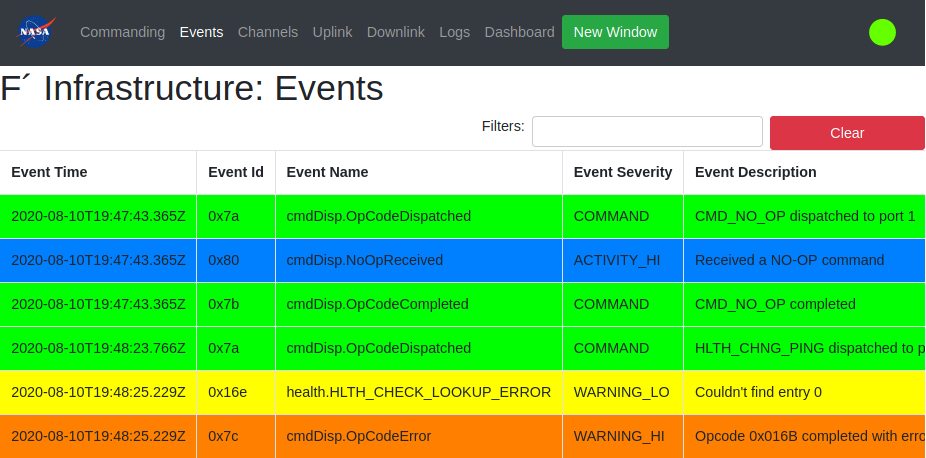
\includegraphics[width=1.0\linewidth]{gds}}
	\caption{Example of FPrime's Ground Data System showing EVRs \cite{b5}.}
	\label{fig:gds}
\end{figure}

FPrime provides an in-browser interface to view EVRs and Tlm as well as send commands directly to the robot. The system, named the Ground Data System (GDS), receives packets transmitted by the robot to a server hosted by the same machine running GDS. The is the developer's main interface to the robots current status, logs, and commanding. Fig. \ref{fig:gds} shows the EVR menu in GDS with various of the event severity levels. This is a live feed from the robot and is transmitted to GDS with a tunneled connection protocol (TCP) connection to the GDS server.

This software framework was selected as it was optimal to avoid extra work with debugging and allowed most of the focus of the project to lie on the design of the vision and navigation subsystems.

\end{comment}

\subsection{Bill of Material}

%TODO

\begin{table}[htb]
	\renewcommand{\arraystretch}{1.2}
	\begin{tabularx}{\columnwidth}{|>{\raggedright\arraybackslash}X|c|}
		\hline
		Part & Price (\$)\\
		\hline
		Raspberry Pi Camera Module V2 & 46.00 \\\hline
		Pastall Raspberry Pi Camera Cable & 7.99 \\\hline
		Standard M12 Thread Interface 180° Fisheye Lens, 1.44mm 1/2.5 Wide Angle & 16.08 \\\hline
		LoveRPi Performance Heatsink & 4.31\\\hline
		Servo Steering Arms & 17.99\\\hline
		Motor Driver RB-WAV-77 & 28.99\\\hline
		Chassis Kit ROB0170 & 98.75\\\hline
		Brushed Motor Kit KIT0167 & 25.00\\\hline
		MG996R 55g Metal Gear Torque Digital Servo & 18.88\\\hline
		Reusable Zip Ties Assorted Sizes & 18.99\\\hline
		UCTRONICS 0.96 Inch OLED Module 12864 128x64 Yellow Blue SSD1306 & 6.99\\\hline
		Tenergy 7.2V Battery Pack for RC Car & 39.99\\\hline
		Sourcingpower Universal RC Battery Charger for 3.6V-9.6V & 19.99\\\hline
		MSP432P401R & 30.00\\\hline
		Raspberry Pi 3B & 42.63\\\hline
		Beato PCB adapter for motor driver & 10.00\\\hline
		\textbf{Total} & 413.59 \\\hline
	\end{tabularx}
	\label{tab:bom}
\end{table}

\section{Proposed Method}

\begin{comment}
This section will discuss the implementation details of the software and hardware of the car. This section will reference the code found in a Github repository: \url{https://github.com/Kronos3/vo-cmpe460.git}. It will be important to first discuss the layout of the code.

The component implementation files discussed in this paper will be found in `Rpi'. Every subdirectory found here will model a separate component. This is with the exception of `Top' that will provide the FPrime topology to initialize and interconnect all of the components. `Top' also includes the main entry point of the software which will perform the nominal boot-up sequence.

Components must provide define their message ports used to interface with other components. These definitions live in the `ComponentNameComponentAi.xml' file that is shipped with every component. Components may also optionally define parameters, events, telemetry, and commands which can be found in their corresponding `.xml' file. These files are inputs into FPrime's automatic programming (autocoding) \cite{b4}. FPrime's autocoding will provide the generic boilerplate code such as
component base classes. The developer will then extend these autocoded base classes with access to the autocoded EVRs and Tlm.

Reusable sequences used to set up the system or run certain algorithms can be found in the `seqs' directory. These files are FPrime sequences have a very simple syntax:

\begin{verbatim}
R00:00:10 component.COMMAND ARG1 ARG2
\end{verbatim}

This command will wait 10 seconds and then dispatch `COMMAND' to `component'. FPrime scripting is used to build the vision pipeline as well as set up a video live stream and begin the navigation algorithm.
\end{comment}

\subsection{Hardware}

The car operates with two compute boards. As previously mentioned, an MSP432P401R microcontroller is used to provide the PWM signals the motors. There are two throttle motors on the rear wheels and a single servo that will control the servo arms. The Raspberry Pi runs the rest of the software that controls the camera and performs communication with GDS.

\begin{figure}[htb]
	\centering
	\centerline{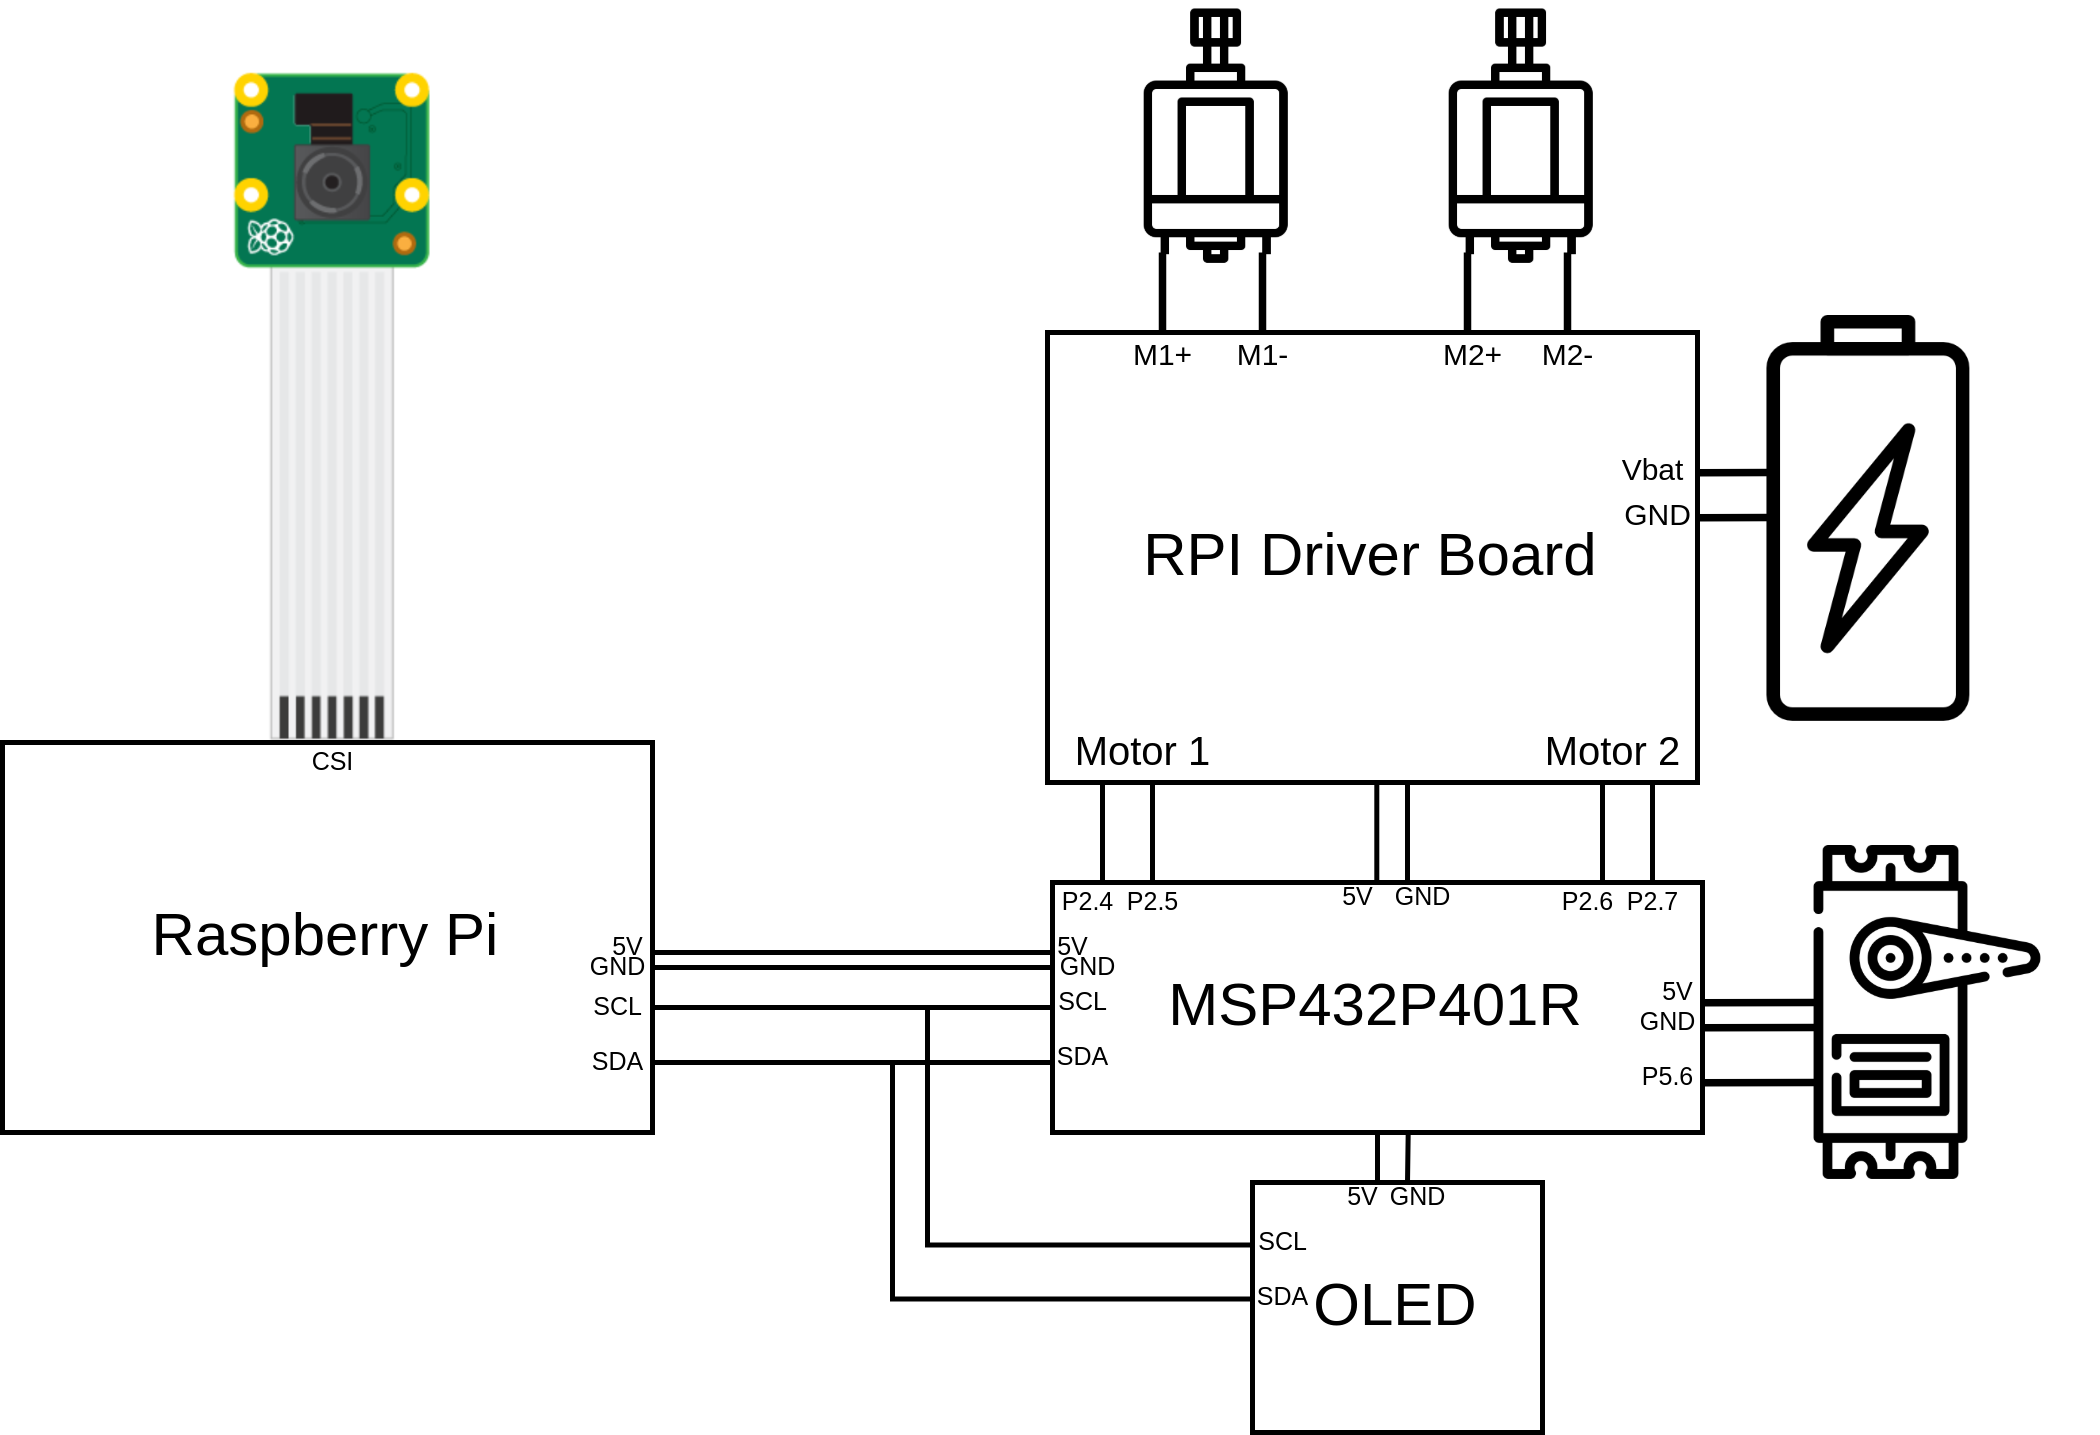
\includegraphics[width=1.0\linewidth]{wiring}}
	\caption{Hardware wiring of Raspberry Pi, MSP432P401R and other hardware.}
	\label{fig:hardware}
\end{figure}

Fig. \ref{fig:hardware} shows the basic wiring scheme of the car. An Inter-Integrated Circuit (I2C) connection is used to send commands from the Raspberry Pi to the MSP432P401R. An organic light-emitting diode (OLED) display is also connected to the common I2C bus. The display is used to print the internet protocol (IP) address of the Raspberry Pi on boot-up so that a user will know where to shell into via a secure-shell (SSH) connection. The Raspberry Pi is the master device in the I2C chain. The Pi is able to arbitrate the common I2C bus by providing the device's unique address before each packet. This will allow the Pi to command both the OLED display and MSP432P401R via the same I2C interface.

The Raspberry Pi Camera Module shown in the upper left corner of Fig. \ref{fig:hardware}, is connected via a ribbon cable to the Pi's Camera Serial Interface (CSI). Due to field-of-view (FOV) limitations of the default camera module's lens, a Fisheye lens with $180^{\circ}$ FOV is used.

\begin{figure}[htb]
	\centering
	\centerline{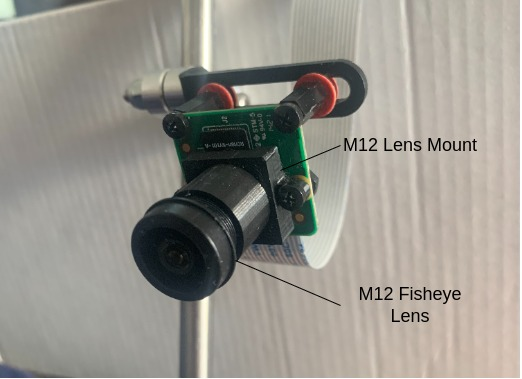
\includegraphics[width=0.7\linewidth]{camera_annotated}}
	\caption{Camera lens and mount.}
	\label{fig:camera}
\end{figure}

Fig. \ref{fig:camera} shows the physical configuration of the fisheye lens
with the camera module. The M12 lens mount shown in Fig. \ref{fig:camera} is a 3D printed lens mount meant for the M12 thread present on the lens in use. Although this lens will cause considerable distortion, it is vital to use a high horizontal FOV lens to be able to see both edges of the track immediately next to the car. The default lens on the camera module has a horizontal FOV of $53^{\circ}$ \cite{b6}. A small horizontal FOV causes the cameras viewport to cut off the peripheral vision the car needs for this application.

\subsection{Component Topology}

This section will discuss the general layout and interaction between all the system components. Also the vital components are discussed though there are many other supporting builtin FPrime components that are not shown. Connections between components indicate some relationship and flow of data.

\begin{figure}[htb]
	\centering
	\centerline{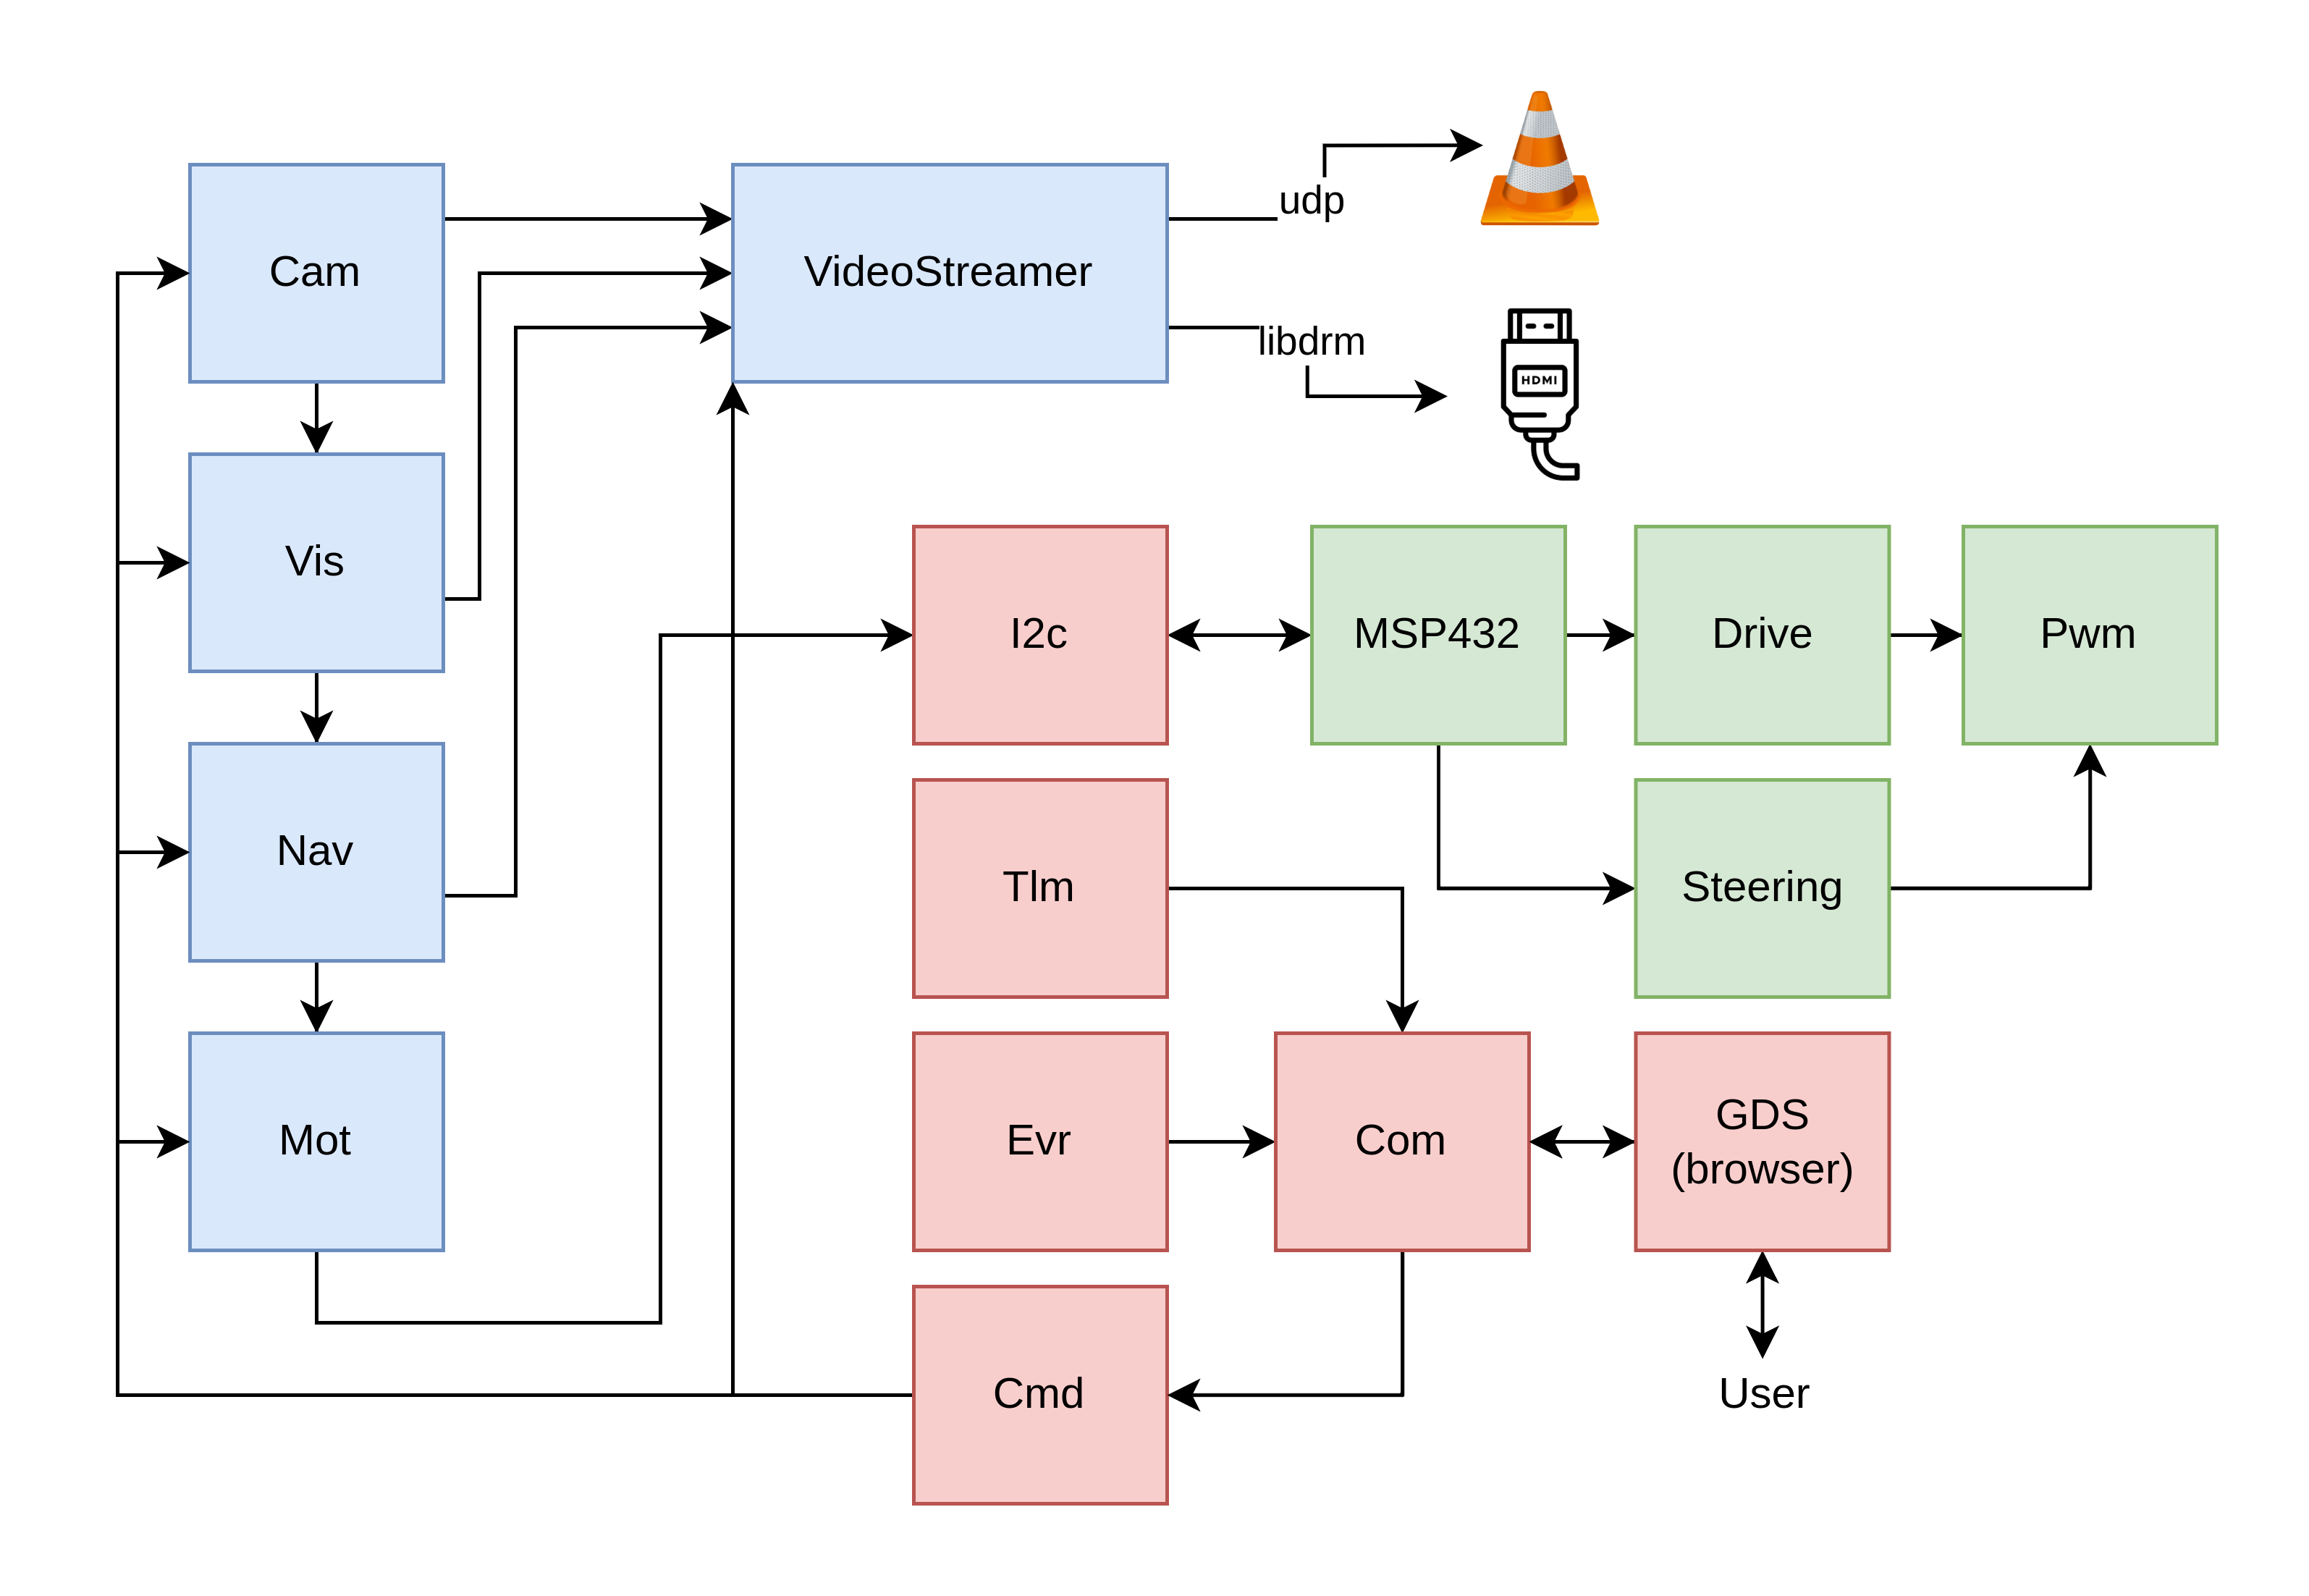
\includegraphics[width=1.0\linewidth]{block}}
	\caption{Full system component topology.}
	\label{fig:block}
\end{figure}

Fig. \ref{fig:block} shows the basic component layout of the project. The camera will acquire image frames and is able to stream to the VideoStreamer or the vision component (Vis). Similarly, Vis is able to stream to the VideoStreamer or to the navigation component (Nav). The video streamer is a component that is able to draw image frames on an HDMI display or to encode a sequence of frames as an H.264 video live stream. This live stream can be viewed externally by a VideoLAN (VLC) media player client. The VideoStreamer is imperative to development and debugging as image frames may be annotated to show algorithms in action.

The MSP432P401R microcontroller is connected to the I2C bus and, as discussed before, will provide the motor control for the DC and servo motor. Both the steering and the dc modules are small wrappers around the pwm module. The pwm module will interface with the TimerA peripheral on-board the MSP432P401R to generate hardware triggered PWM waves.

\subsection{Motor (Mot)}

The microcontroller's sole purpose in this design is to control the motors. The Raspberry Pi needs a communication protocol for encoding command packets sent to the microcontroller. The `Mot' component will handle this interaction by encoding a command packet and sending it out over the I2C bus. A command packet will consist of two single byte fields: opcode and value. Opcodes denote a specific command such as `left\_forward' or `right\_backward' and will take an argument in the value field.

Mot will allow control from other components via a more generic synchronous
messaging port. The steering port will allow floating point values from $-1$ (left) to $1$ (right), while the throttle port will allow two throttle values from $-1$ (backwards) to $1$ forwards for each of the two DC motors. Mot is therefore responsible for encoding a software friendly floating point number, to a hardware friendly command packet to send to the microcontroller.

\subsection{Camera (Cam)}

The camera component (Cam) is responsible for interfacing with the camera. This software will use libcamera to interface directly with the kernel driver and hardware. Once a camera stream is initialized, Cam will need to manage the camera buffers sent and received from the camera. Frame acquisition requests can be made to the camera by queuing frame buffer for the camera to work with. When an image is acquired, the camera will send a filled image buffer back to Cam and Cam will then send out the frame to a registered listener.

Looking at Fig. \ref{fig:block}, Cam, Vis, Nav, and VideoStreamer are all interconnected. These connections refer to image frames being passed through the components via asynchronous messaging. It is the responsibility of each component to either pass the image frame to another component, or to return the image frame to the Cam. When the frame is returned to the Cam, it is reused for acquisition by placing on the frame buffer queue.

For use with the car, the camera will capture 1640x1232 pixel image frames at 30 frames per second (FPS). The camera's saturation is zeroed as a gray-scale image is used for image processing. The white balance is set to auto which will help calibrate the color balance in different room environments.

\begin{comment}
\subsection{VideoStreamer}

VideoStreamer is a very simple component that is able to display image frames on select-able mediums. The VideoStreamer supports displaying to a High-Definition Multimedia Interface (HDMI) connected directly to the Pi or to stream over the network to a VideoLAN Client (VLC) using a UDP connection. The HDMI display is able to draw memory-mapped Direct Memory Access (DMA) memory regions which are specially allocated by the Linux kernel. These memory mapped regions can be written to and read from directly by the integrated graphics processing unit (GPU). Camera frame buffers also must reside in these memory mapped regions as the Raspberry Pi camera will apply hardware accelerated post-processing before releasing the image to the camera client. This means that the original image buffer provided by the camera process must be passed directly to the HDMI streaming process and the buffer must be held until another frame is ready to display. This logic because quite complex in terms of managing the life cycle of each frame buffer. When a frame buffer is no longer in use, it must return to the camera to acquire a new frame. To keep track of when a frame buffer is in use, a reference counter is used to keep track of the lifetime of the buffer. This idea is the Python programming language uses to keep track the life cycle of its objects \cite{c7}.

Because HDMI is only useful in the early stages of development, a separate display method is used to transmit encoded video over the network. Transmitting each individual raw frame over the network would be extremely inefficient and provide for poor results. Instead, the video is encoded into an H.264 video stream and transmitted over the network via a UDP connection. The VideoStreamer will leverage the Raspberry Pi's hardware H.264 video encoder via the videodev2 library to provide accelerated encoding capabilities. Although in noisy environments the UDP stream may occasionally be interrupted briefly, the H.264 encoder and UDP connections are able to keep up with the framerate requirements presented by this project.

\end{comment}

\subsection{Vision (Vis)}

The Vis component is possibly the most important component in the robot. The purpose of this component is to process the image frame in such a way that the navigation component can use it for controlling the car. Vision will receive raw image frames from the camera and apply a series of transformations to the image. Each transformation is known as a pipeline stage where the culmination of all the stages is known as the pipeline.

The entire pipeline in Vis is completely modular. This means that the pipeline stages can be added or the entire pipeline cleared via a set of sequence commands. Pipeline stages may have parameters associated with them which can similarly be set via command. This modular design allows for easy changes to be made to the vision pipeline as well as allowing multi-purpose use of the vision component. For example, a race vision pipeline can be initialized during the race boot-up sequence to perform edge detection. Similarly, a calibration pipeline can be set up to compute the camera pose and be used for perspective correction. Another advantage of this method is simplicity in implementation. Each pipeline stage is an extremely simple processing step and therefore reduces the chance of programming errors.

\subsubsection{Edge Detection}

When designing the race pipeline, the input into the navigation must be considered. The purpose in the Vis component is to apply transformations to the image that will provide Nav with information to place itself on the track. For this project, the most important features to extract from the image frame are the edges of the track. We would therefore expect Vis to transform the raw image to only include track lines. This can be done with an edge detector.

\begin{figure}[htb]
\begin{minipage}[b]{.48\linewidth}
	\centering
	\centerline{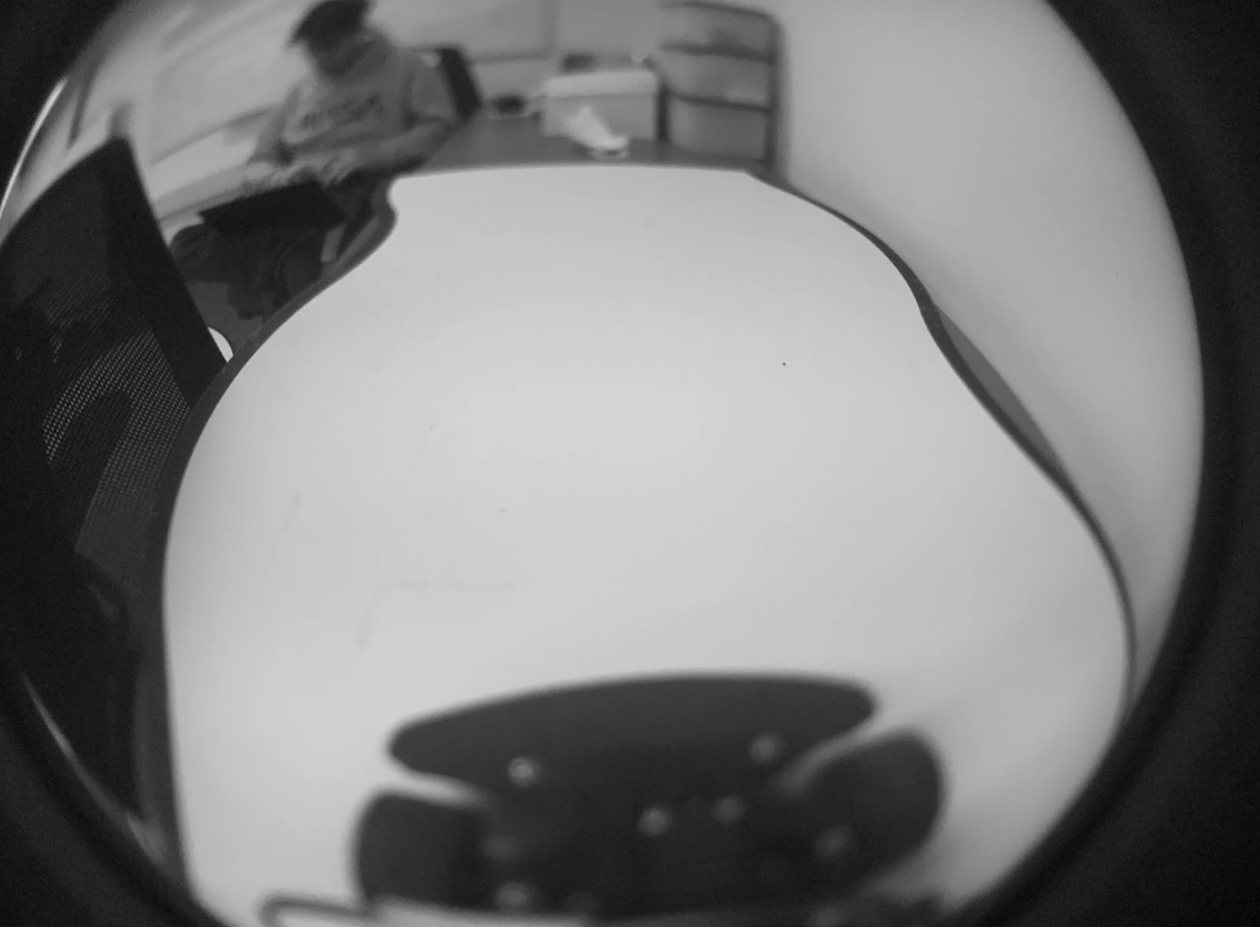
\includegraphics[width=4.0cm]{vis_figs/raw}}
	%  \vspace{1.5cm}
	\centerline{(a) Raw image}\medskip
\end{minipage}
\hfill
\begin{minipage}[b]{0.48\linewidth}
	\centering
	\centerline{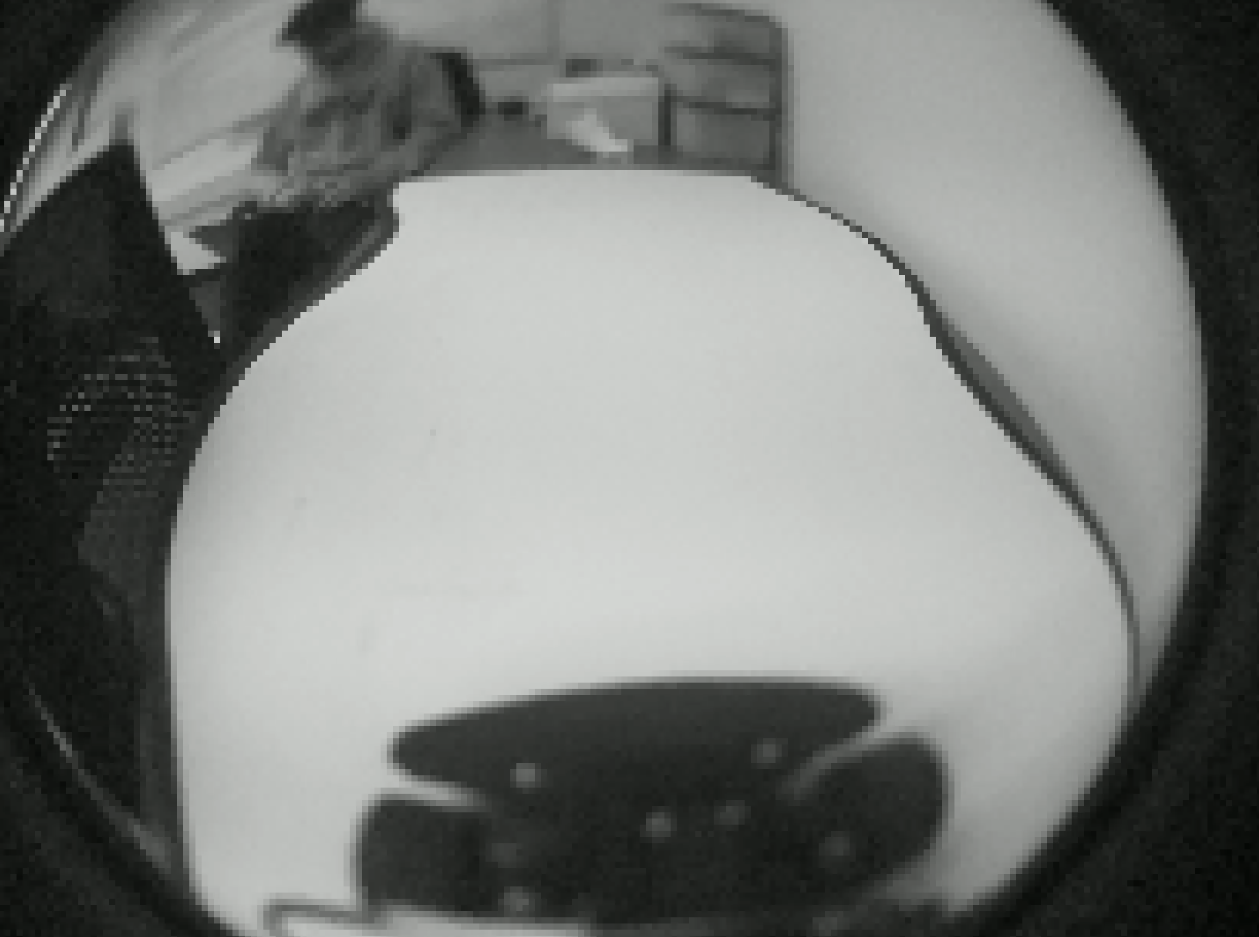
\includegraphics[width=4.0cm]{vis_figs/downscale}}
	%  \vspace{1.5cm}
	\centerline{(b) Downscale (x16)}\medskip
\end{minipage}
%
\begin{minipage}[b]{.48\linewidth}
	\centering
	\centerline{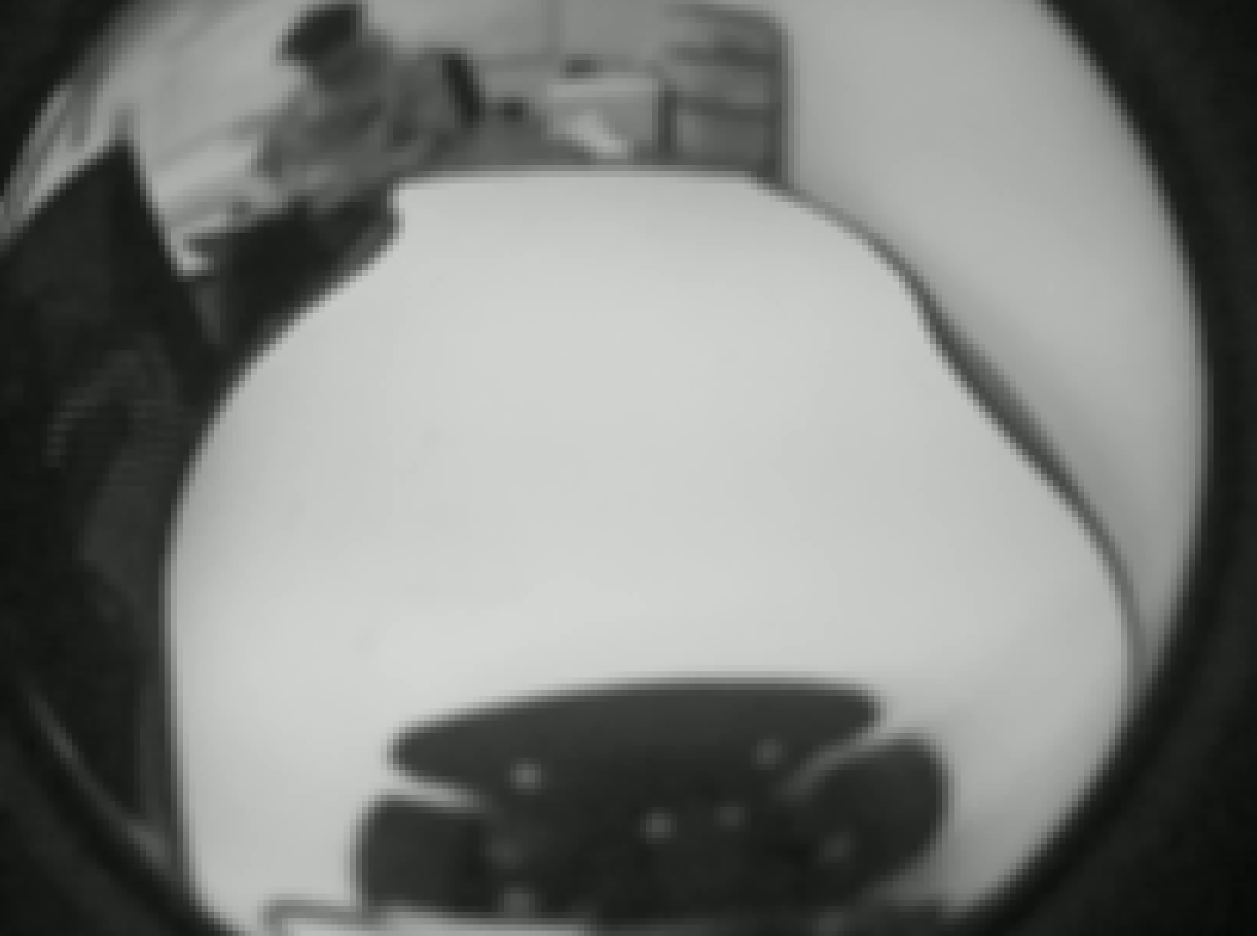
\includegraphics[width=4.0cm]{vis_figs/gaussian}}
	%  \vspace{1.5cm}
	\centerline{(c) Gaussian blur}\medskip
\end{minipage}
\hfill
\begin{minipage}[b]{0.48\linewidth}
	\centering
	\centerline{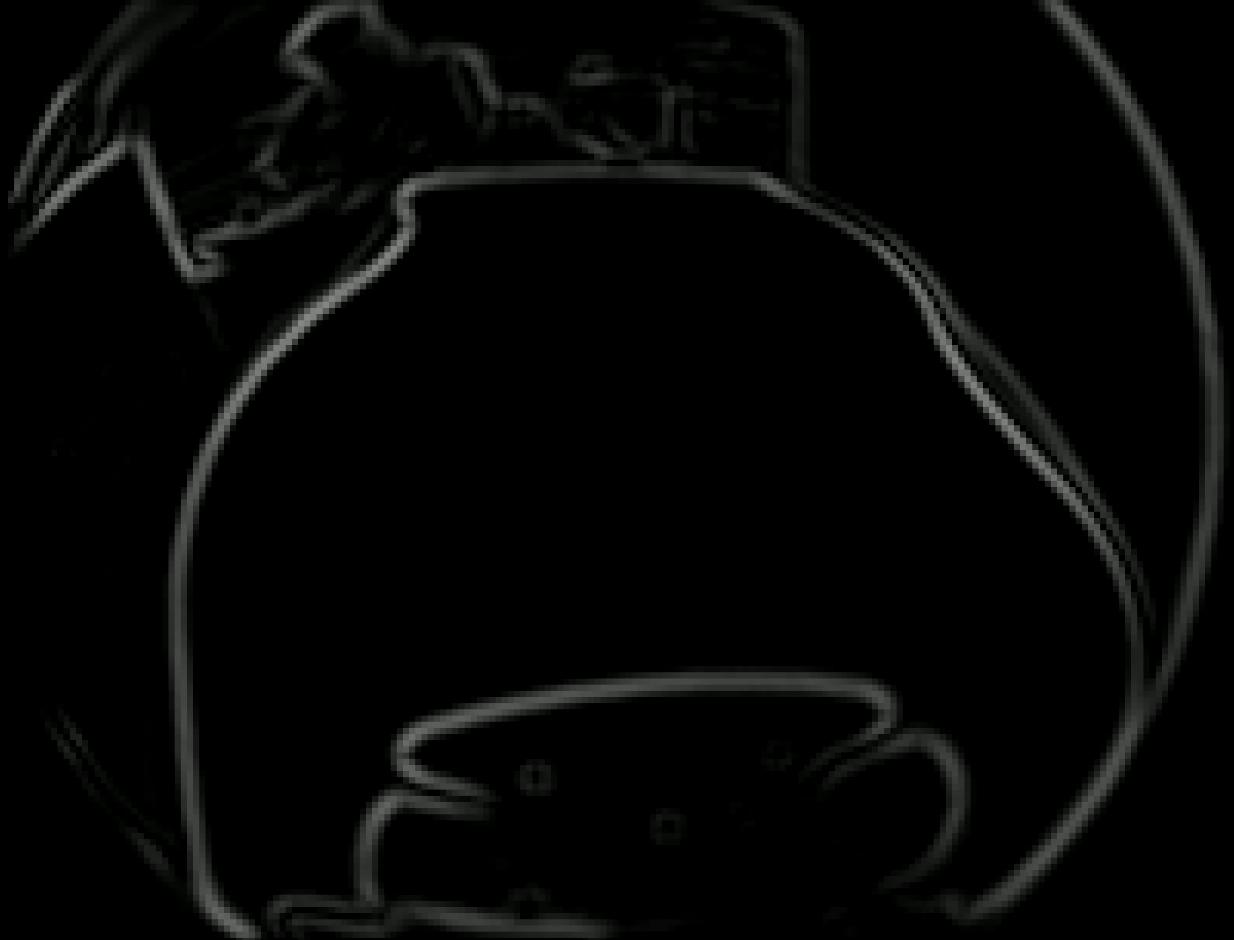
\includegraphics[width=4.0cm]{vis_figs/gradient}}
	%  \vspace{1.5cm}
	\centerline{(d) Sobel XY edge filter}\medskip
\end{minipage}
%
\caption{First four stages of the race pipeline applied to the
	same image.}
\label{fig:vis1}
%
\end{figure}

Fig. \ref{fig:vis1} shows an image of the car on a section of the track. This test is especially interesting because the track is next to a white wall. With a 16x downscale (Fig. \ref{fig:vis1} (a))applied to the image, it is even for the human eye to make out the edges of the track. The Sobel filter however is able to appropriately find these edges using its convolution kernel by applying filter similar to a 2 dimensional gradient. The purpose in applying a Gaussian blur filter to the image before the Sobel filter is to essentially apply a low pass digital filter. This will smooth out noisy regions as well as make track edges thicker get rid of small gaps in the line edges. Like the Sobel filter, the Gaussian blur is a convolution kernel however, instead of applying a gradient functor, a weighted average of surrounding pixels is used. This racing pipeline will use a 3x3 kernel Gaussian blur as it has reasonable computational performance and yields an acceptable output.

\subsubsection{Pose Calibration}

When working with camera's on robots, it is very common to calibrate the pose of the camera \cite{b1} \cite{b3}. This refers to computing the rotation and translation matrix relative to a known point on the ground plane. Calibrating the pose would allow the image frame to be transformed into "birds-eye" view orientation. This orientation is obviously advantageous to the navigation algorithm as its easier to form a navigational path when looking directly above. Depth estimation on a planar surface is trivial when looking directly from above.

OpenCV supports pose calibration via its calib3d library. This project uses a chessboard calibration target as it is the most commonly used target for pose calibration. This is simply a set of black squares on white paper tapped to a piece of cardboard and layed out in-front of the car. OpenCV is able to find the corners between the squares and provide the user with a set of image coordinates. Because these corners are at known positions on the calibration target, OpenCV is able to derive pose information from the location of the these squares.

\begin{figure}[htb]
	\centering
	\centerline{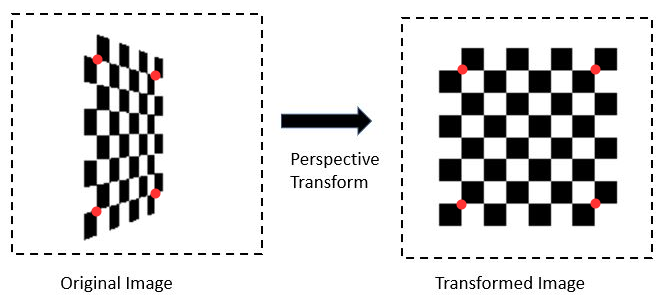
\includegraphics[width=1.0\linewidth]{perspective_annotated}}
	\caption{Perspective transform applied to chessboard image.}
	\label{fig:perspective}
\end{figure}

Fig. \ref{fig:perspective} shows an example of a chessboard with a perspective transform applied to it. To build the transformation matrix, two sets of four points must be provided. The first set of points lies on the raw image and maps out the input plane of the transform. The second set of points will lie on the transformed frame which in this case, should be evenly spaced to warp the image to birds-eye view.

\begin{figure}[htb]
	\begin{minipage}[b]{.48\linewidth}
		\centering
		\centerline{\includegraphics[width=4.0cm]{vis_figs/vis\_intersection}}
	\end{minipage}
	\hfill
	\begin{minipage}[b]{0.48\linewidth}
		\centering
		\centerline{\includegraphics[width=4.0cm]{vis_figs/vis\_straight}}
	\end{minipage}
	\caption{Vis processed images of intersection and straightaway.}
	\label{fig:vis2}
\end{figure}

The full vision pipeline's results shown in Fig. \ref{fig:vis2} show a combination of processing done in Fig. \ref{fig:vis1}, a warp transform, and finally a binary threshold to create hard edges. Fig. \ref{fig:vis2} shows very good results near the center of the image with relatively straight lines on the straightaway (right). The distortion around the edges of the frame are caused by lens distortion from the fish-eye lens. Fish-eye lens distortion is a common problem in robot that require a large FOV such as \cite{b1}. The distortion can be corrected with the calibrated camera model discussed above. This transform however is too computationally intensive for the Raspberry Pi and cannot maintain a stable frame stream for the navigation step.

\subsection{Navigation (Nav)}

The final step to control the car is to ingest Vis processed image frames and to derive a desired path around the track. The idea here is to find points on the track edge and build a spline that draws out the edges of the track.

\subsubsection{Line \& Center classification}

The classification of track lines is a relatively in-depth process. A method that utilizes OpenCV's contour finding HoughLinesP algorithm was initially investigated. This path was immediately dropped as the algorithm was far too slow to be used for realtime contour classification and can only be used on straight lines. This project uses an iterative algorithm to trace lines and find track edges.

\begin{figure}[htb]
	\begin{minipage}[b]{.48\linewidth}
		\centering
		\centerline{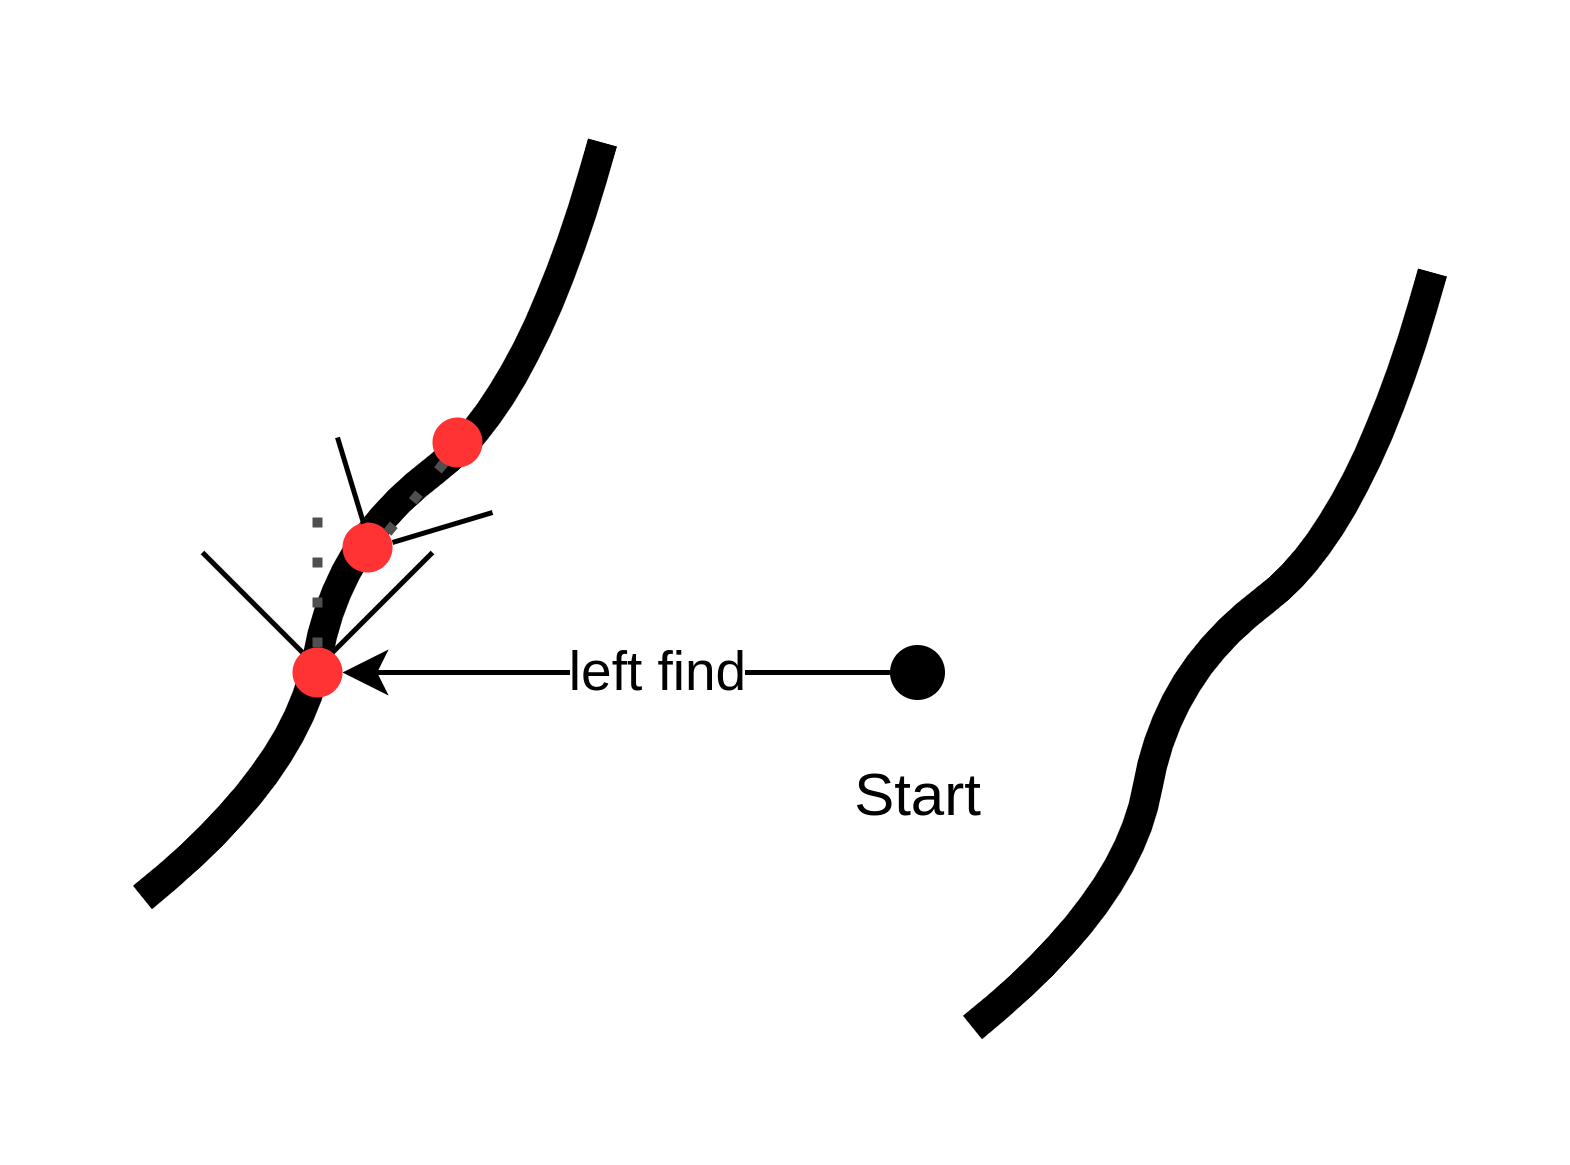
\includegraphics[width=4.0cm]{track}}
	\end{minipage}
	\hfill
	\begin{minipage}[b]{0.48\linewidth}
		\centering
		\centerline{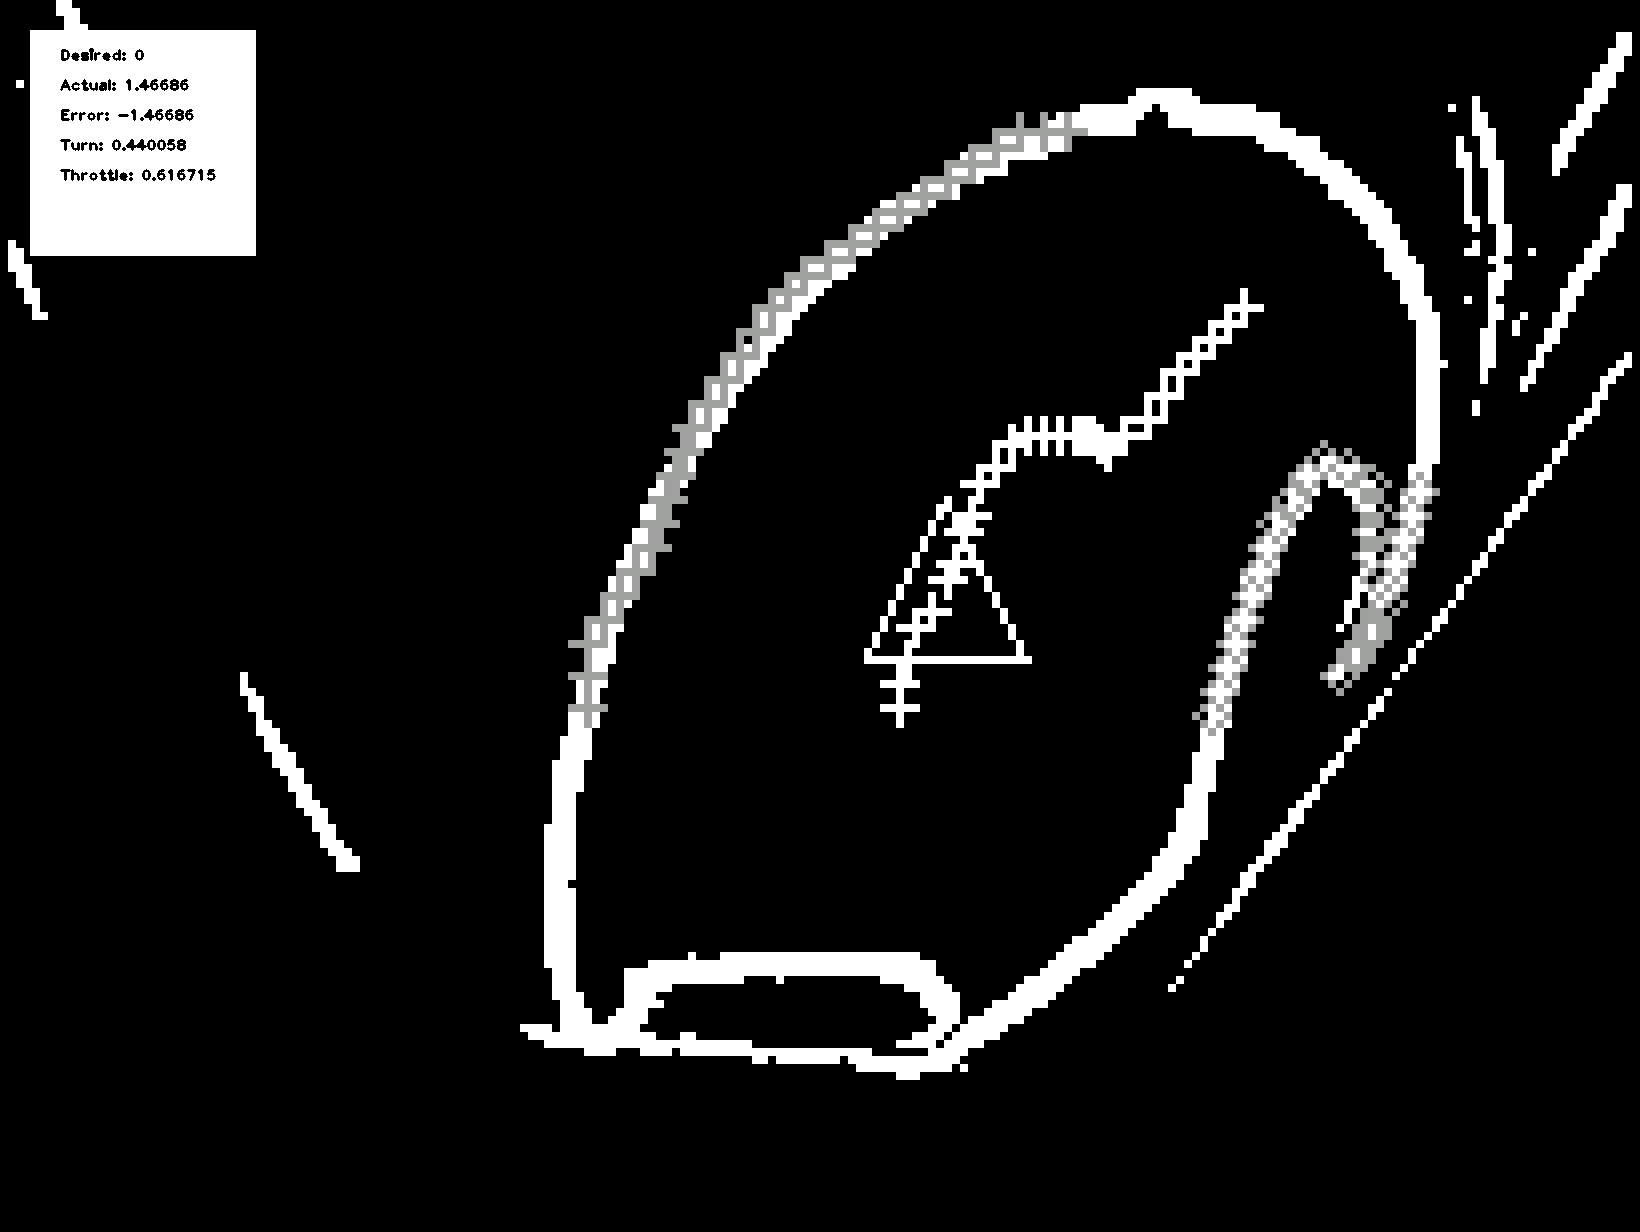
\includegraphics[width=4.0cm]{vis_figs/nav_turn}}
	\end{minipage}
	\caption{Vis processed images of intersection and straightaway.}
	\label{fig:track_find}
\end{figure}

Fig. \ref{fig:track_find} shows the basic idea behind the iterative algorithm used for line classification. A configurable start point on the image is used to search for the left and right track lines. A linear search for the edge is performed for both left and right edges. When they are found, a step process is used to trace along the path of the line. The next point is found by searching along a circle of configurable radius out from the current point. Fig. \ref{fig:track_find} left shows three lines protruding from the detected point. The center dotted line is the start search angle which will be equal to the angle that the last point is found at. The solid lines represent the angle restrictions placed on the angle sweep search. By iterating along this search path, a set of points can trace the track lines. with relatively high accuracy.

Although the track lines can be detected well, the center line is more difficult to classify. Fig. \ref{fig:track_find} right attempts to draw a center through the detected track edges. The left and right track edges were properly detected with a fairly high degree of accuracy. Center points are derived by simply averaging the points from the left and right sides of the track. This evidently cannot work as the outer edge of the track will have a longer arc than the inner edge of the track. A similar method attempts to find the center line by approximating the track edges as 2D parametric splines. Theoretically, by tracing a normal line from one of the edge, the line will intersect with the opposite point on the track. In practice however, the distortion due to the fish-eye lens causes the normals to lack this mathematical property. The result of a poorly mapped center line makes it difficult to control the car through turns.


\begin{comment}
\subsubsection{Center classification}

Nominally, Nav should be able to see both edges of the track and derive a center line. The center line being the control basis for the PID control scheme.

\begin{figure}[htb]
	\centering
	\centerline{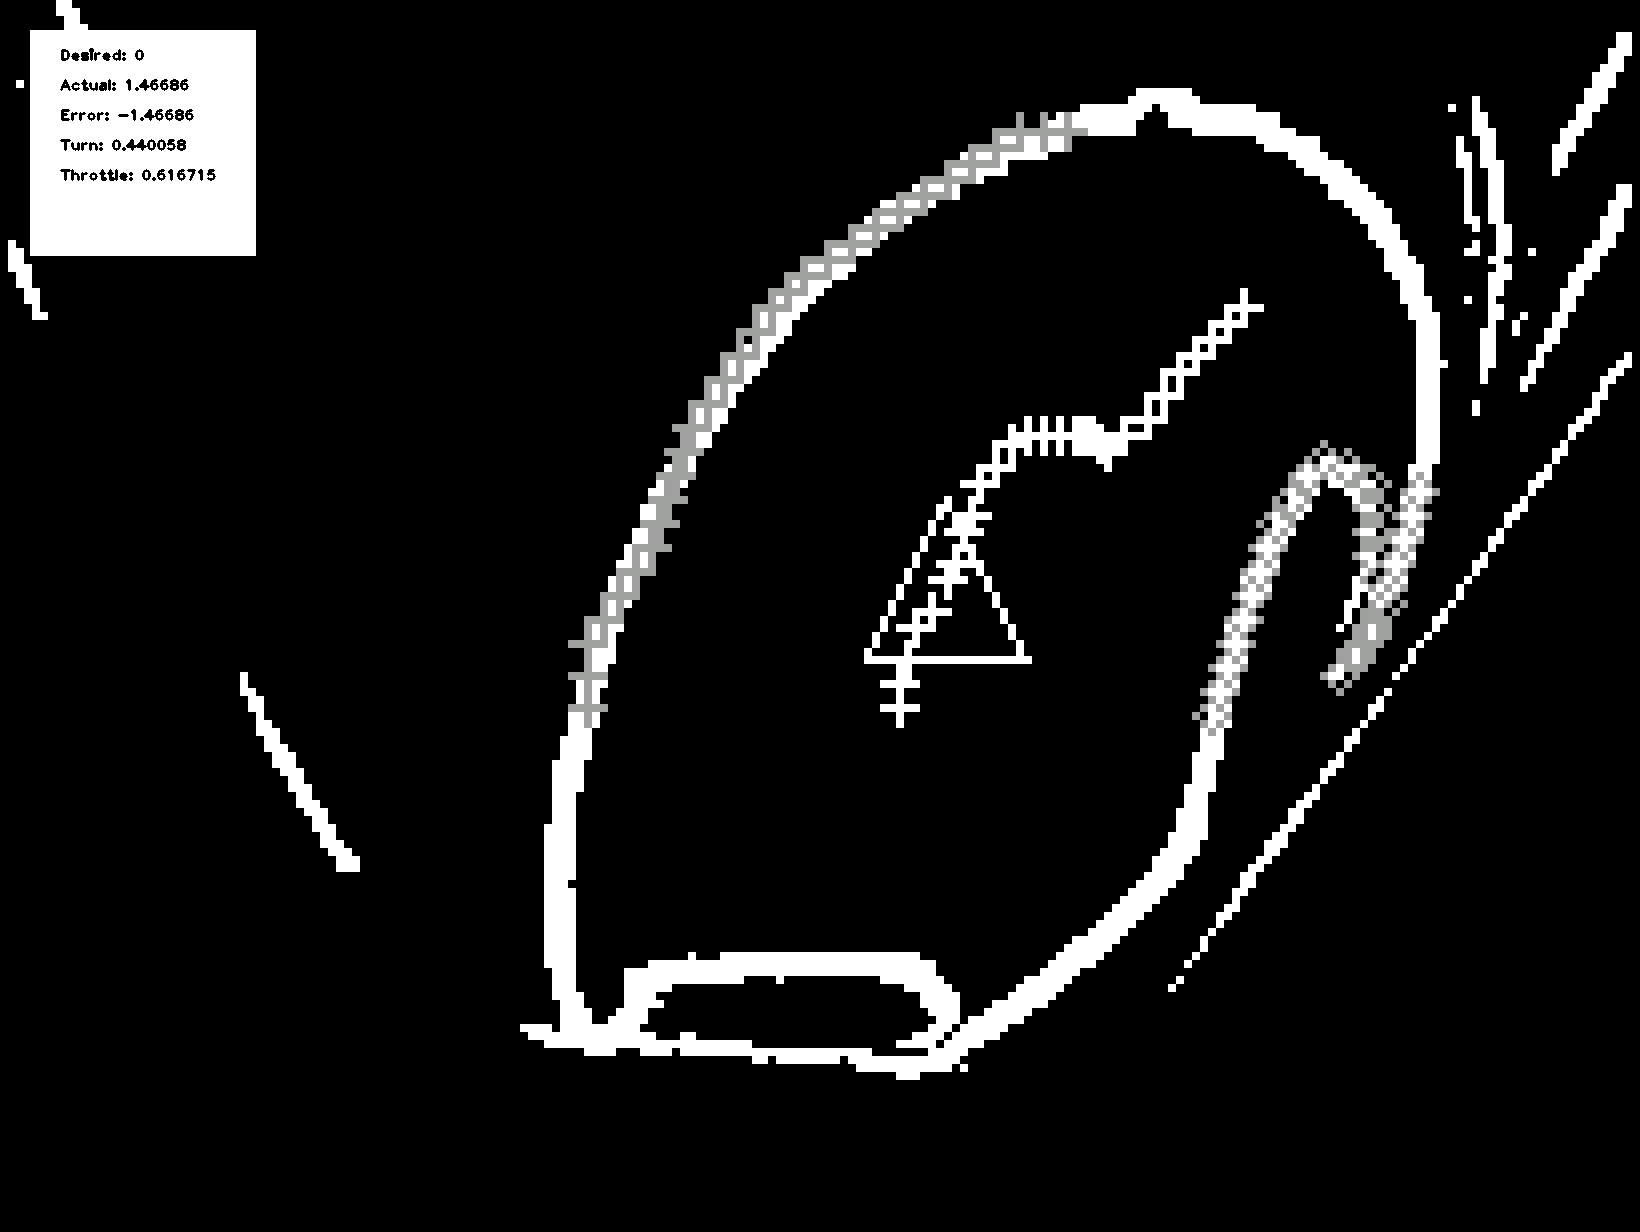
\includegraphics[width=1.0\linewidth]{vis_figs/nav_turn}}
	\caption{Nav annotations applied to Vis processed image frame.}
	\label{fig:nav_turn}
\end{figure}

Fig. \ref{fig:nav_turn} attempts to draw a center through the detected track edges. The left and right track edges were properly detected with a fairly high degree of accuracy. Center points are derived by simply averaging the points from the left and right sides of the track. This evidently cannot work as the outer edge of the track will have a longer arc than the inner line of the track. Another method similar to this way attempted by approximating the points as a set of 2D splines. These splines were parametric splines where the parameter was normalized by the arc length between each set of points. This however yielded similar results to those shown in \ref{fig:nav_turn}. No reliable form of center classification was found though future work is discussed later in this paper.

Another method attempted during this step was to follow a normal line from the outer edge. Theoretically, by tracing a normal line away from one of the edge, the line will intersect with the opposite point on the track. The center of this normal line will correspond to one of the center points of the track. This method however is not viable as the distortion due to the fisheye lens causes the line normals to lack this mathematical property. An undistort would need to be applied before attempting this method. As previously mentioned, undistortion of images using the camera calibration matrix is too computationally intensive for the Raspberry Pi and therefore this method was abandoned.

\end{comment}

\subsubsection{PID Control}

The final control of the car is done by providing a PID process with a current error estimate. Using the perspective transform, the center of the image corresponds to the center line of the car. By looking at the track's center line derived in the previous step, we can derive the distance the car is from the center of the track. Depending on the current speed of the car, points on the center line may be used to derive an error estimate.

The PID controller can be tuned to adjust the response of the car given error over time. PID parameters can be set via command and saved to disk using FPrime's parameter database. Because the center line classification is so unreliable in the corners, a good set of PID parameters was never found.

\section{Results}

Although the car could travel very slowly (around 25 DC duty cycle) around a simple track, the navigation of the car suffered from a host of problems that caused the final product to not be ready for race day. This section of the paper looks to discuss what went wrong, what went right, as well as provide possible future work that could improve the performance of the car.

\subsection{What went wrong}

One of the issues seen throughout many portions of this project was performance. Although many steps were taken to minimize the effect of the low compute power of the Raspberry Pi, all four Pi cores were running at maximum load when the race pipeline was processing frames. Performance issues attempted to be solved by downscaling the raw image frame. While this worked for many of the linear and convolutional operators, an undistort operation for correcting fish-eye lens distortion could never be added to the pipeline.

Although performance was an issue, the main problem in this project was the overall complexity of the navigation. While the vision pipeline provided surprisingly good images with little more than track edges showing, the chosen navigation algorithm was not reliable for every track configuration and car orientation. The car could handle well on straight portions and single turns however suffered from misclassification of track lines when multiple turns were chained together.

\subsection{What went right}

Although ultimately the car never started the race, many portions of this project were successful. The motor control across the I2C bus was also built to be robust and could handle packet sending errors if a physical connection was unreliable. The camera and vision system were designed well and worked with little flaws. There was a lot of work that went into getting a reliable raw stream from the camera as well as encoding the video stream and transmitting it over the network. Much of the time in this project was spent getting the basic features working. This took time away from developing a reliable navigation algorithm.

Finally, the downlink capabilities for EVRs and telemetry as well as uplink of command sequences and dispatch were essential in providing a high quality development environment. This capability made it possible to quickly build and test new vision pipeline features as well as set parameters for certain stages. Without the modular design of the Vis component and the capabilities of the FPrime framework, this project would never have gotten as far as it did.

\subsection{Future work}

Much of the framework and features on this project are not likely to be changed significantly in the future. The Cam, Vis, Mot, and VideoStreamer are all fairly well thought out and do not require any significant redesign. To make this car operate at its full potential, the method for navigation needs to see further work. Possible routes for improvement include applying an adaptive threshold instead of an edge detector to classify raw image pixels as `track' and `no-track'. This may eliminate the performance issues as well as possibly providing a navigation algorithm a simpler processed frame to work with.

Another future design change could implement a neural net control system. A neural net could be relatively easy to train using the framework already in place. A game controller could be used to manually drive the car around a track and provide the net with training data. The net could be further refined by providing elapsed time feedback to the learning algorithm that could further adjust pathing. A neural net could work in tandem with the vision system already in place and would simply work with a smaller region of interest to improve performance.

Finally, the choice of a Raspberry Pi was mostly due to the hardware availability of the board. Ideally, the NVIDIA Jetson Nano computer would be used which includes a similar software configuration to the Raspberry Pi and the presence of a enormously more powerful 472 giga-floating-point-operations-per-second (GFLOPS) GPU \cite{b8}. By comparison, the Raspberry Pi's four cores can produce about 3.62 GFLOPS \cite{b2}. The Nano also does not suffer from virtually non-existent documentation for its GPU which makes it far more supported in open source tools such as OpenCV.

\section{Conclusion}

The Raspberry Pi control car 

\begin{thebibliography}{00}
\bibitem{b1} J. N. Maki, D. Gruel, “The Mars 2020 engineering cameras and microphone on the Perseverance Rover: A next-generation imaging system for mars exploration - space science reviews,” SpringerLink, 24-Nov-2020. [Online]. Available: https://link.springer.com/article/10.1007/s11214-020-00765-9. [Accessed: 20-Apr-2022]. 
\bibitem{b2} “Power consumption benchmarks,” Power Consumption Benchmarks | Raspberry Pi Dramble. [Online]. Available: https://www.pidramble.com/wiki/benchmarks/power-consumption. [Accessed: 18-Apr-2022].
\bibitem{b3} A. Rosebrock, “Raspberry Pi For Computer Vision,” PyImageSearch, 08-May-2021. [Online]. Available: https://pyimagesearch.com/2019/04/05/table-of-contents-raspberry-pi-for-computer-vision/. [Accessed: 18-Apr-2022].
\bibitem{b4} R. L. Bacchino, T. K. Canham, G. J. Watney, L. J. Reder, and J. W. Levison, “F Prime: An Open-Source Framework for Small-Scale Flight Software Systems,” NASA JPL Beacon, 04-Aug-2018. [Online]. Available: https://trs.jpl.nasa.gov/handle/2014/48425. [Accessed: 20-Apr-2022]. 
\bibitem{b5} “A brief guide to the F´ ground data system,” F´. [Online]. Available: https://nasa.github.io/fprime/UsersGuide/gds/gds-introduction.html. [Accessed: 20-Apr-2022].
\bibitem{b6} “Raspberry pi documentation,” Camera. [Online]. Available: https://www.raspberrypi.com/documentation
/accessories/camera.html. [Accessed: 20-Apr-2022].
\bibitem{c7} “Reference counting,” Reference Counting - Python 3.10.4 documentation. [Online]. Available: https://docs.python.org/3/c-api/refcounting.html. [Accessed: 23-Apr-2022].
\bibitem{b8} “Jetson modules,” NVIDIA Developer, 22-Mar-2022. [Online]. Available: https://developer.nvidia.com/embedded/jetson-modules. [Accessed: 25-Apr-2022]. 
\end{thebibliography}

\setlength{\columnsep}{8pt}
\setlength{\intextsep}{0pt}
\begin{wrapfigure}{L}{0.20\textwidth}
	\centering
	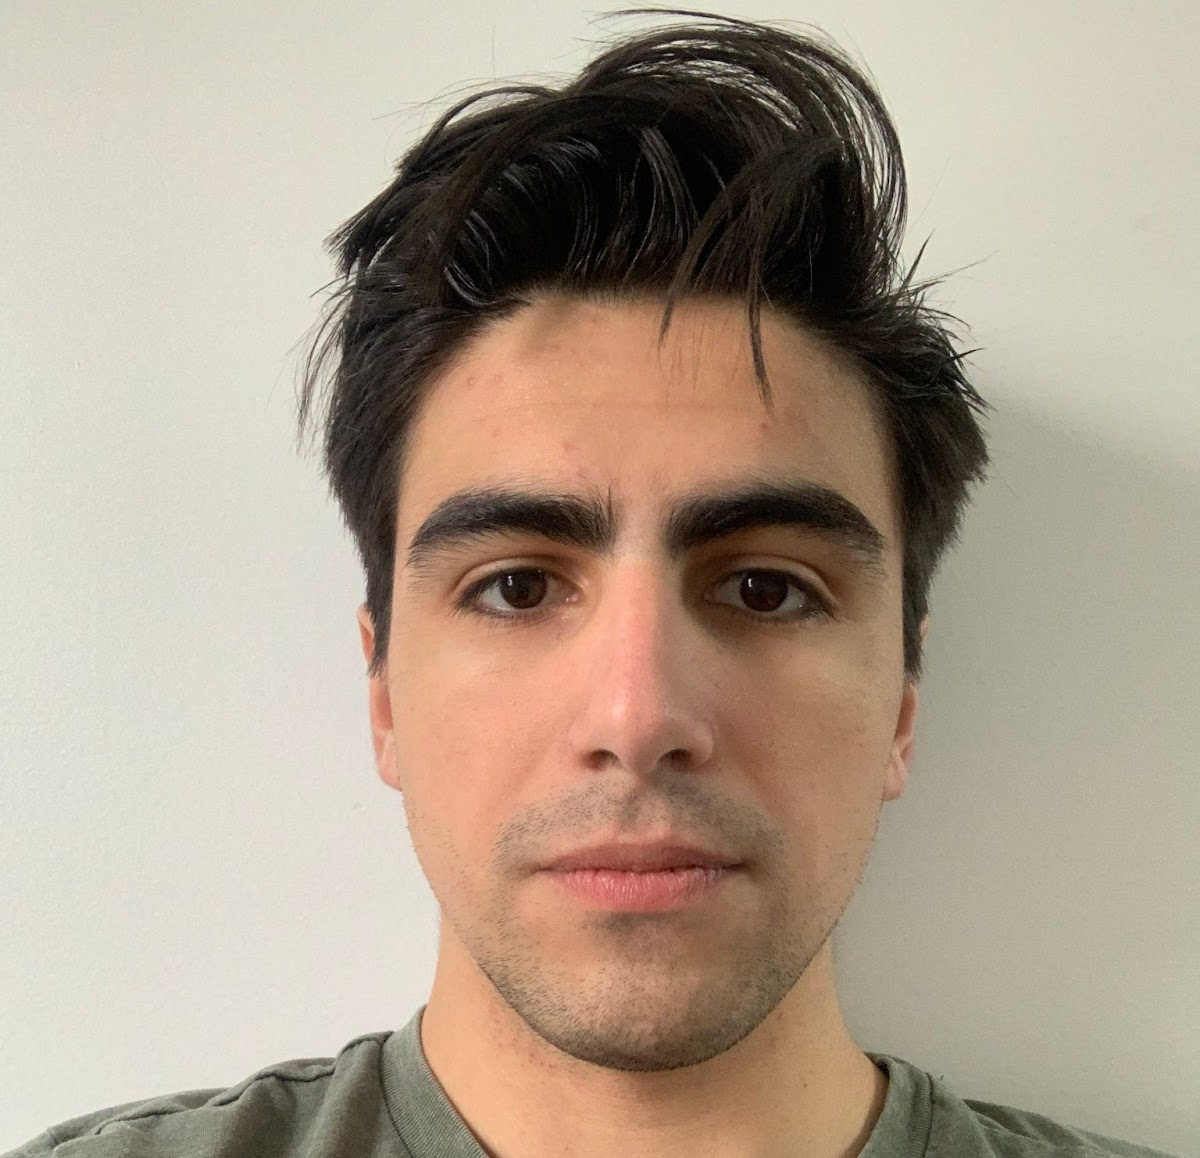
\includegraphics[width=0.20\textwidth]{author}
\end{wrapfigure}
\noindent
\textbf{Andrei Tumbar} is a third year Computer Engineering student in Kate Gleason College of Engineering at Rochester Institute of Technology. He has been working for NASA Jet Propulsion Laboratory for two years in the Robotic Operations group. Andrei has been building operations tools for Perseverance, Curiosity, ColdArm, Ingenuity, as well as a contributor to the FPrime Flight-Software framework. He is interested in robotics, embedded systems, and has a newfound interest in computer vision.

\begin{comment}
\begin{authorbiography}{author}
	{Andrei Tumbar}
	is a third year Computer Engineering student in Kate Gleason College of Engineering at Rochester Institute of Technology. He has been working for NASA Jet Propulsion Laboratory for two years in the Robotic Operations group on Perseverance, Curiosity, ColdArm, Ingenuity, as well as a contributor to the FPrime Flight-Software framework. He is interested in robotics, embedded systems, and has a newfound interest in computer vision. 
	is a third year Computer Engineering student in Kate Gleason College of Engineering at Rochester Institute of Technology. He has been working for NASA Jet Propulsion Laboratory for two years in the Robotic Operations group on Perseverance, Curiosity, ColdArm, Ingenuity, as well as a contributor to the FPrime Flight-Software framework. He is interested in robotics, embedded systems, and has a newfound interest in computer vision.
\end{authorbiography}
\end{comment}

\end{document}